\documentclass[
  landscape,
  a0paper,
  20pt,
  margin=0mm,
  innermargin=10mm,
  blockverticalspace=0mm,
  colspace=5mm,
]{tikzposter} % See Section 3
\usepackage{xcolor}
\usepackage[style=authoryear-comp, locallabelwidth]{biblatex}
\addbibresource{bibliography.bib}
\usepackage{amsmath}
\usepackage{xurl}
\usepackage{tabularx}
\usepackage{booktabs}

\newcommand{\actualTitle}{Using Bayesian Regression to Quantify Sexual Dimorphism in Dinosaurs}
\newcommand{\species}[1]{\textit{#1}}
\newcommand{\tyran}{\species{Tyrannosaurus rex}{}}
\newcommand{\psit}{\species{Psittacosaurus lujiatunensis}{}}
\newcommand{\maia}{\species{Maiasaura peeblesorum}{}}
\newcommand{\normal}[2]{\ensuremath{\mathcal{N}\left(#1, #2\right)}}


\renewcommand*{\bibfont}{\tiny}

\title{\actualTitle} % See Section 4.1
\author{Eric Campbell \\ \texttt{eric.robert.campbell@gmail.com}} 
\institute{Calefy Inc.}
\settitle{ \centering \vbox{
\@titlegraphic \\[\TP@titlegraphictotitledistance] \centering
\color{titlefgcolor} {\bfseries \Huge \sc \@title \par}
\vspace*{1em}
{\huge \@author \par} \vspace*{1em} {\LARGE \@institute} \vspace*{1em}

}}
\usetheme{Simple} % See Section 5

\begin{document}
\maketitle[
    width = 0.8\textwidth,
    titletotopverticalspace = 5mm,
    titletoblockverticalspace = 5mm,
  ] % See Section 4.1
\block{Abstract}{While sexual dimorphism is common in extant taxa, detection in extinct taxa is made challenging by difficulties in determining the sex and size of organisms. Existing methods suffer from a lack of statistical power, making positive identification of dimorphism difficult. Herein is outline an modification to a method from \cite{saittaEffectSizeStatistical2020} which constructs sex-specific growth curves to determine sexual size dimorphism, but using Bayesian regression to construct the curves rather than standard non-linear regression. The method is shown to be robust and reliable, with the additional benefit of incorporating prior information to constrain dimorphism to biologically plausible levels.} % See Section 4.2
\begin{columns} % See Section 4.4
\column{0.333333333} % See Section 4.4
\block{Introduction}{
  \begin{itemize}
    \item Sexual dimorphism is common in extant taxa, but positive examples in dinosaurs are rare
    \item Determining sex and size of an extinct organism is difficult
    \item Existing methods suffer from low statistical power and can be confounded by e.g. juveniles
    \item Method in \cite{saittaEffectSizeStatistical2020}: construct growth curves for predicted male and females separately to measure dimorphism
    \item Can suffer from lack of numerical convergence and implausible predictions (e.g. negative masses), particularly for small sample sizes
    \item Proposed modification: use Bayesian regression to estimte growth curves
  \end{itemize}
}
\block{Method}{
  \begin{enumerate}
        \item Gather data: age (or a correlate) and character of interest (e.g. length)
        \item Fit growth curve to population as a whole 
        \item Predict sex by assigning all samples above the population curve to one sex and all below to the other. 
        \item \textcolor{red}{Fit separate growth curves to each predicted sex} $\to$ Create a posterior distribution for sex-specific parameters (Bayesian regression)
        \item \textcolor{red}{Calculate maximum likelihood level of dimorphism} $\to$ Calculate posterior distribution for dimorphism
  \end{enumerate}
  \begin{tikzfigure}[Simulated Alligator Populations \& Method]
    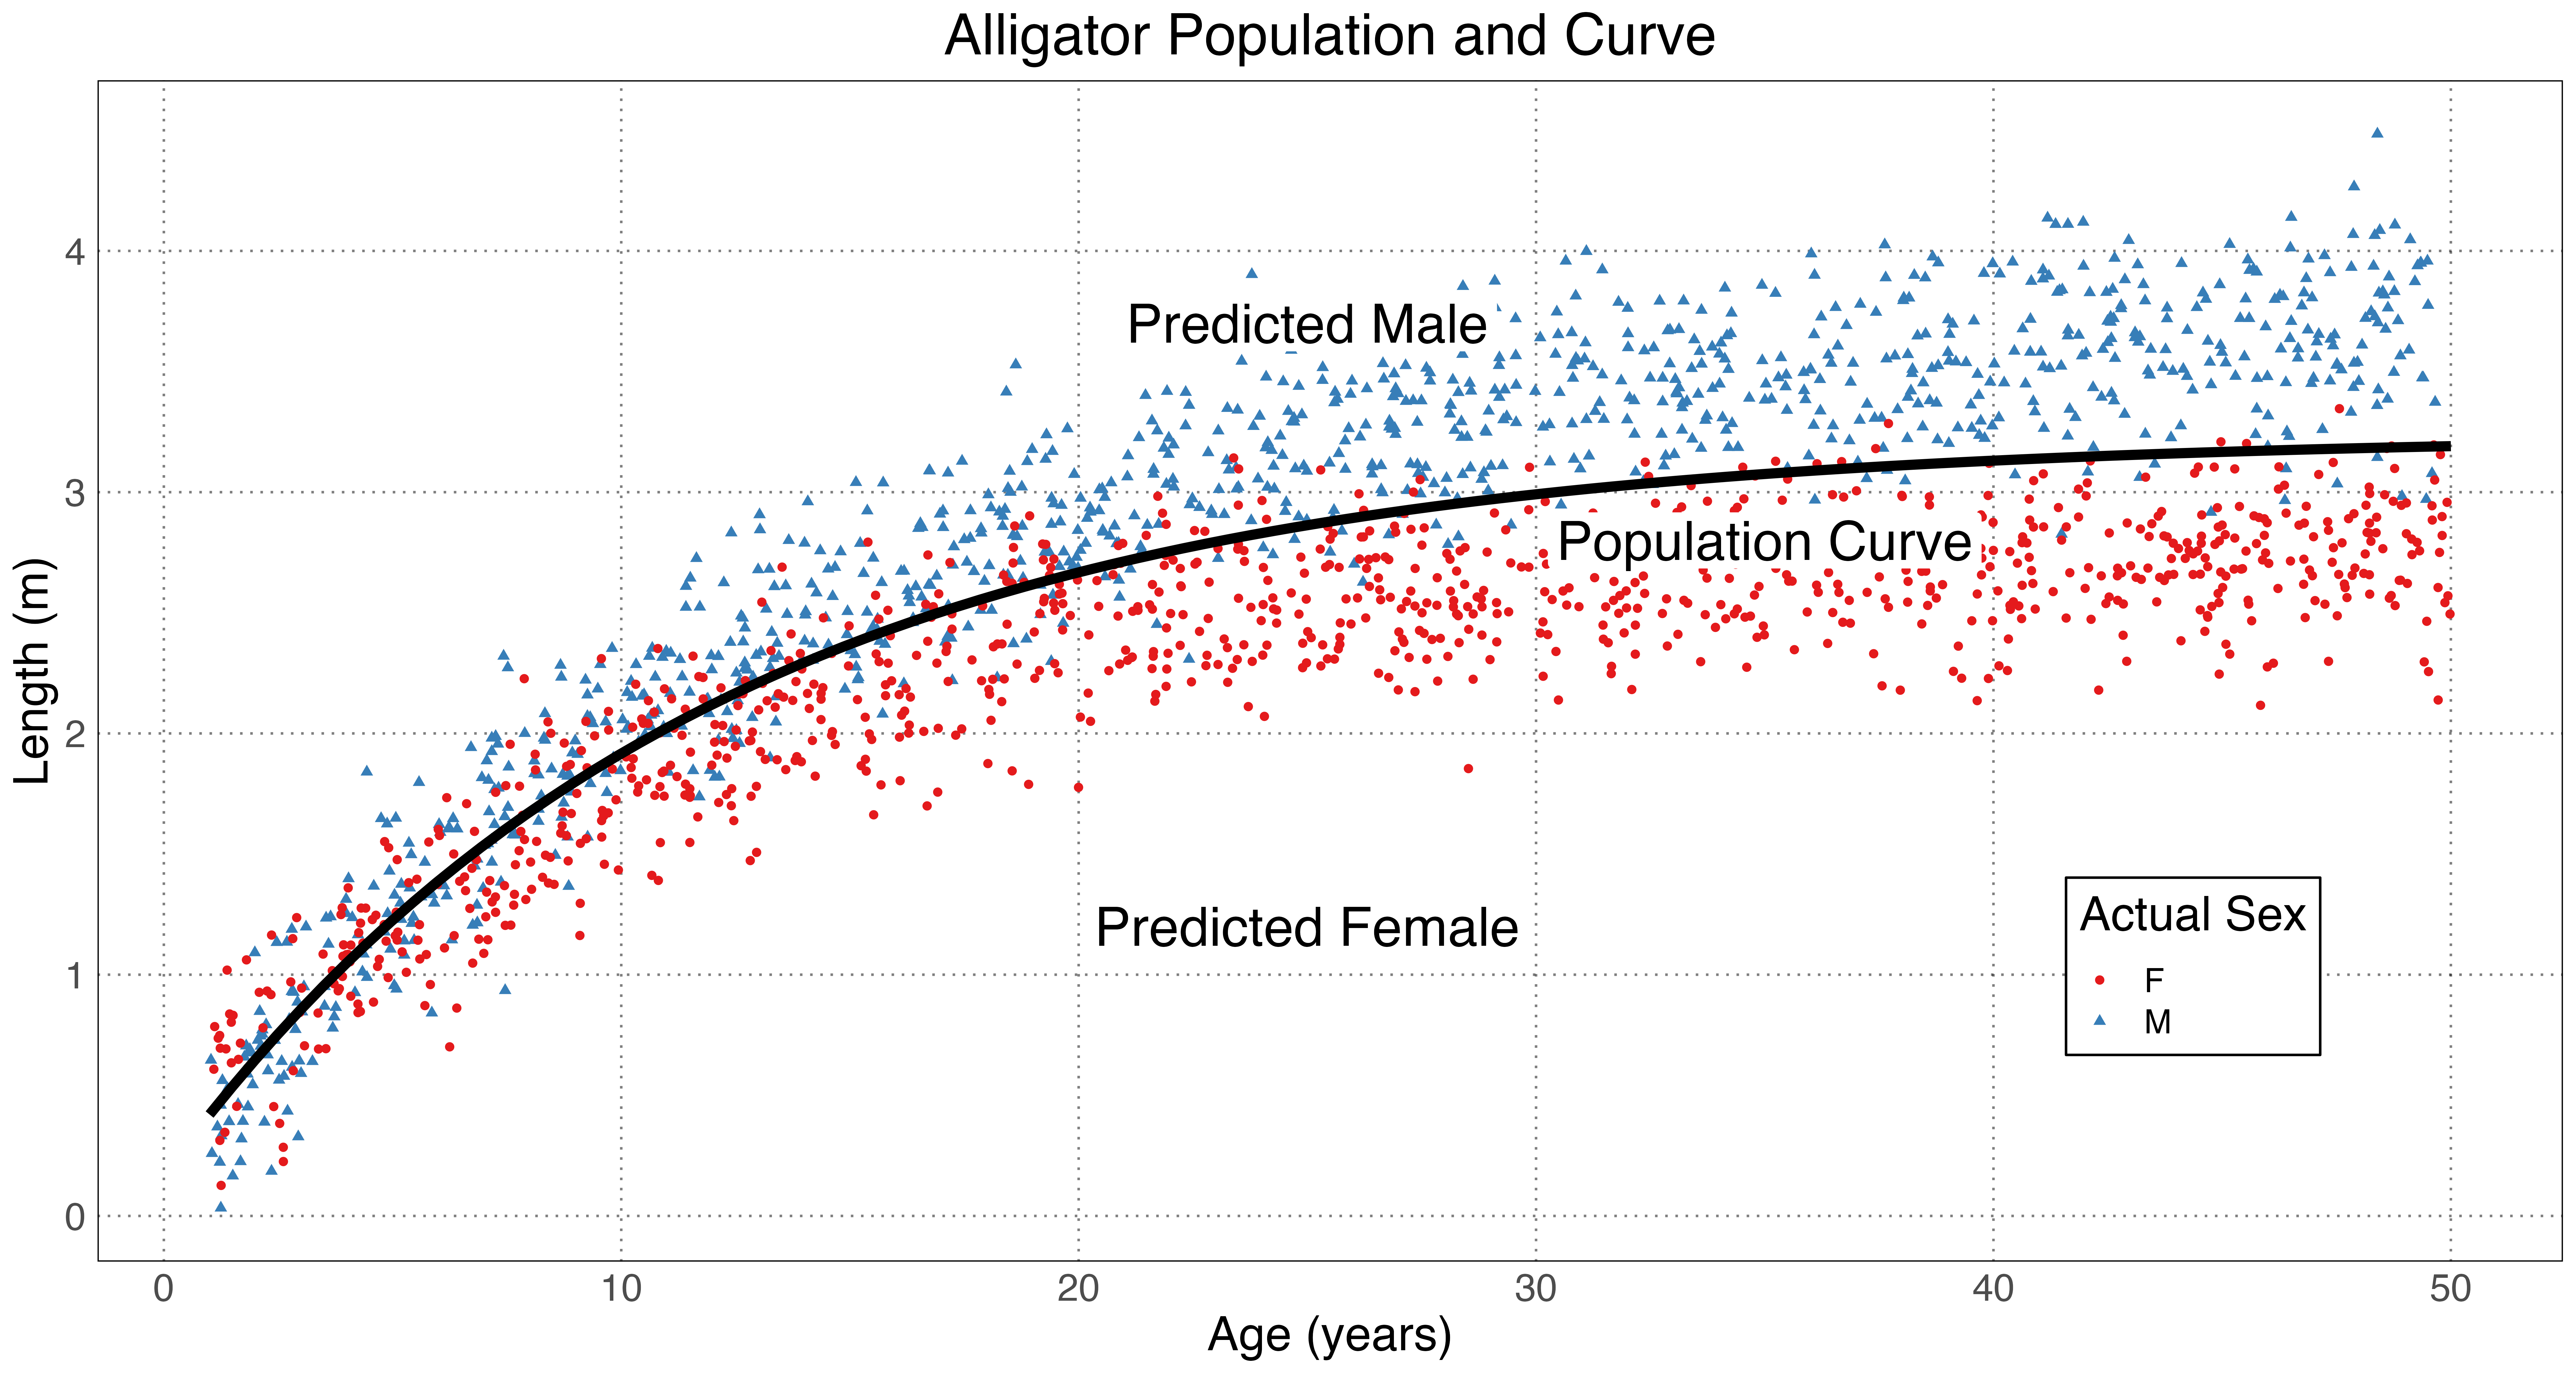
\includegraphics[width = 0.9\colwidth]{images/alligatorMethod-poster.png}
  \end{tikzfigure}
For all data and code used here, along with additional analyses, see \url{https://github.com/EricRobertCampbell/aps-2024-poster-sexual-dimorphism}.
}

\column{0.333333333}
\block{Verification}{
  Bayes' Theorem:
  \[
    \overbrace{P\left(\text{parameter value}|\text{data}\right)}^{\text{Posterior}} \propto \overbrace{P\left( \text{parameter value} \right)}^{\text{Prior}} \ast \overbrace{P \left( \text{data} | \text{parameter value}\right)}^{\text{Likelihood}}
  \]

    \begin{minipage}[t]{0.45\colwidth}
      \begin{tikzfigure}[Bayesian parameter estimation]
        \centering
        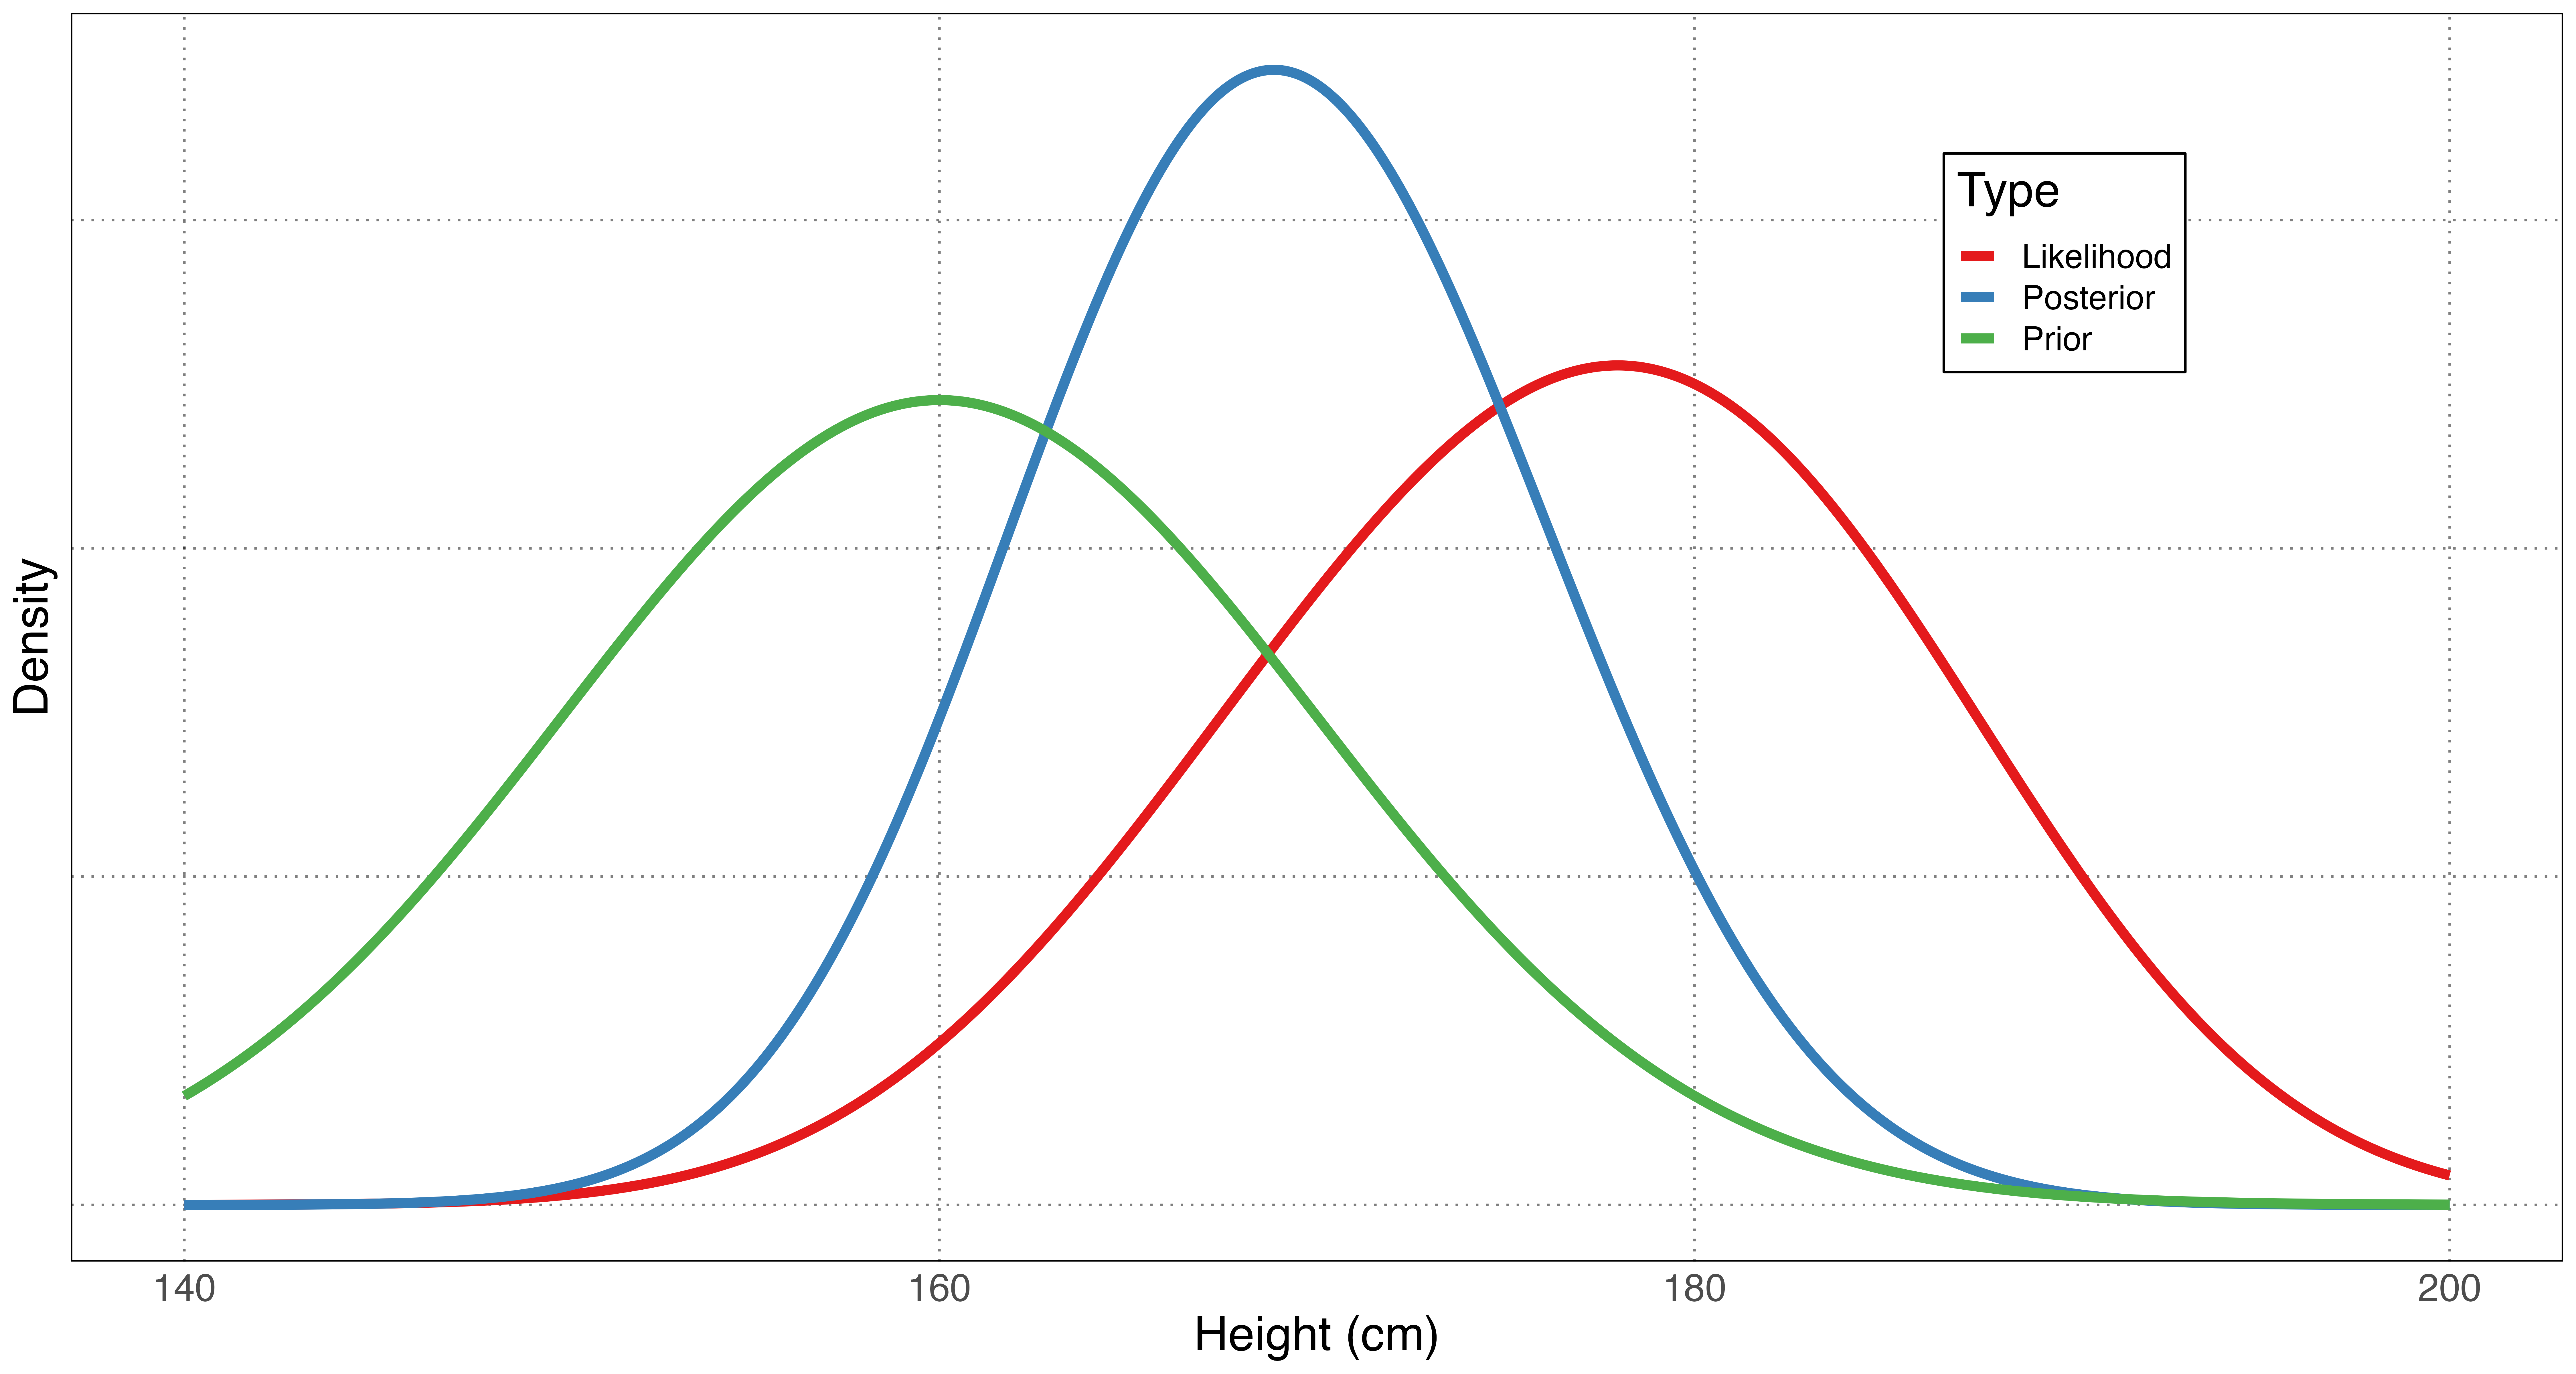
\includegraphics[width = \textwidth]{images/bayesianExample-poster.png}
        \label{fig:bayesianExplanation}
      \end{tikzfigure}
    \end{minipage}
    \begin{minipage}[t]{0.45\colwidth}
      \begin{itemize}
          \item To estimate mean human height, start with what we know about the height before seeing any data --- the \emph{prior}
          \item A sample of heights is collected and the \emph{likelihood} of that sample for each of the potential mean heights is calculated
          \item Combination of those, our final belief about the value of the mean height, is the \emph{posterior} distribution
      \end{itemize}
    \end{minipage}
  \begin{itemize}
    \item American alligator (\species{Alligator mississippiensis}) growth parameters from \cite{wilkinsonGrowthRatesAmerican1997} (von Bertalanffy growth curve), but with constant standard deviation


    \begin{minipage}[t]{0.45\colwidth}
    \section*{Simulated}
    \begin{align*}
    \text{Length}_{ m / f } &\sim \mathcal{N}\left(\mu_{ m / f }, \sigma_{m/f}\right) \\
    \mu_m &= 3.79 * \left(1 - 0.94e^{-0.0695 \ast \text{age}}\right) \\
    \mu_f &= 2.78 * \left(1 - 0.91e^{-0.0926 \ast \text{age}}\right) \\
    \sigma_{m/f} &= 0.25
    \end{align*}
  \end{minipage}
  \begin{minipage}[t]{0.45\colwidth}
    \section*{Model}
    \begin{align*}
    \text{Length}_{m/f,i} &\sim \normal{\mu_{m/f, i}}{\sigma_{m / f}} \\
    \mu_{m/f, i} &= \text{von Bertalanffy}(\text{age}_i, \\
                & L_{ m/f }, A_{ m/f }, K_{ m/f }) \\
    L_{ m/f } &\sim \normal{\text{population L}}{0.5} \\
    A_{ m/f } &\sim \normal{\text{population A}}{0.025} \\
    K_{ m/f } &\sim \normal{\text{population K}}{0.05} \\
    \sigma_{m/f} &\sim \normal{0.25}{0.05} \\
    \end{align*}
  \end{minipage}
    \item Bayesian model with wide priors centred around the population-level curve values was used to recover the values \parencite{rCore, rstan}.

  \end{itemize}
    \begin{tikzfigure}[Verification results]
      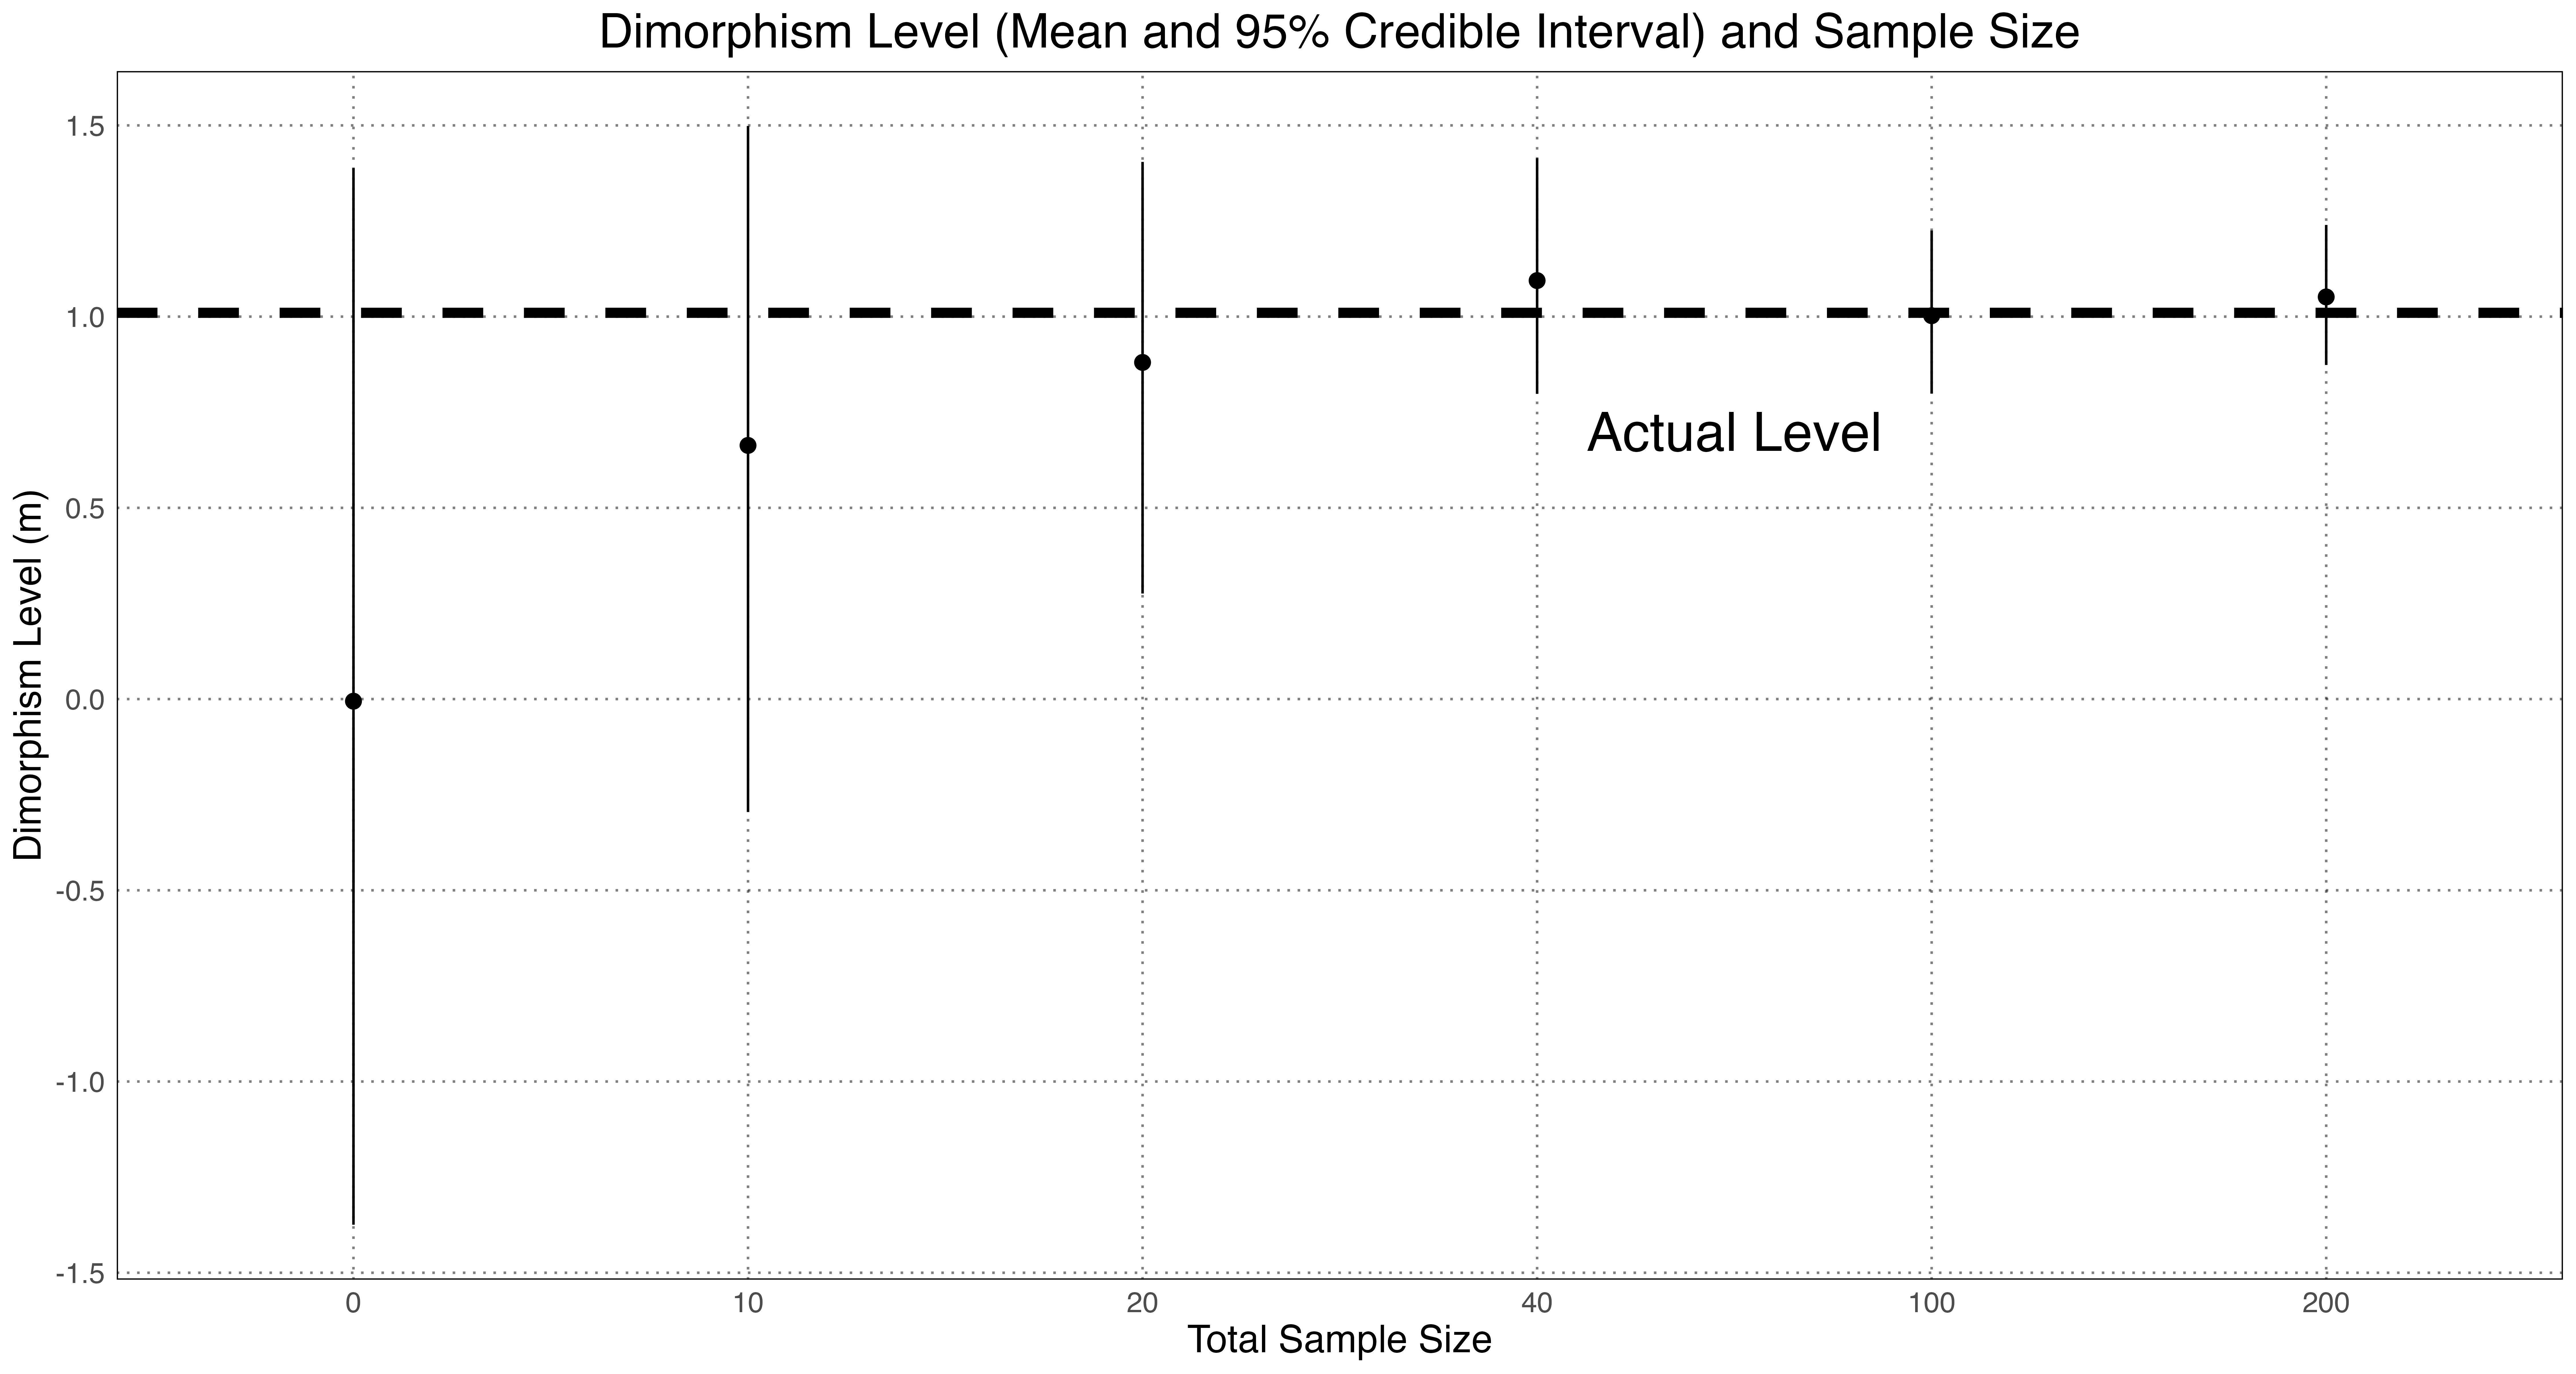
\includegraphics[width = 0.4\colwidth]{images/alligatorSampleSize-poster.png}
      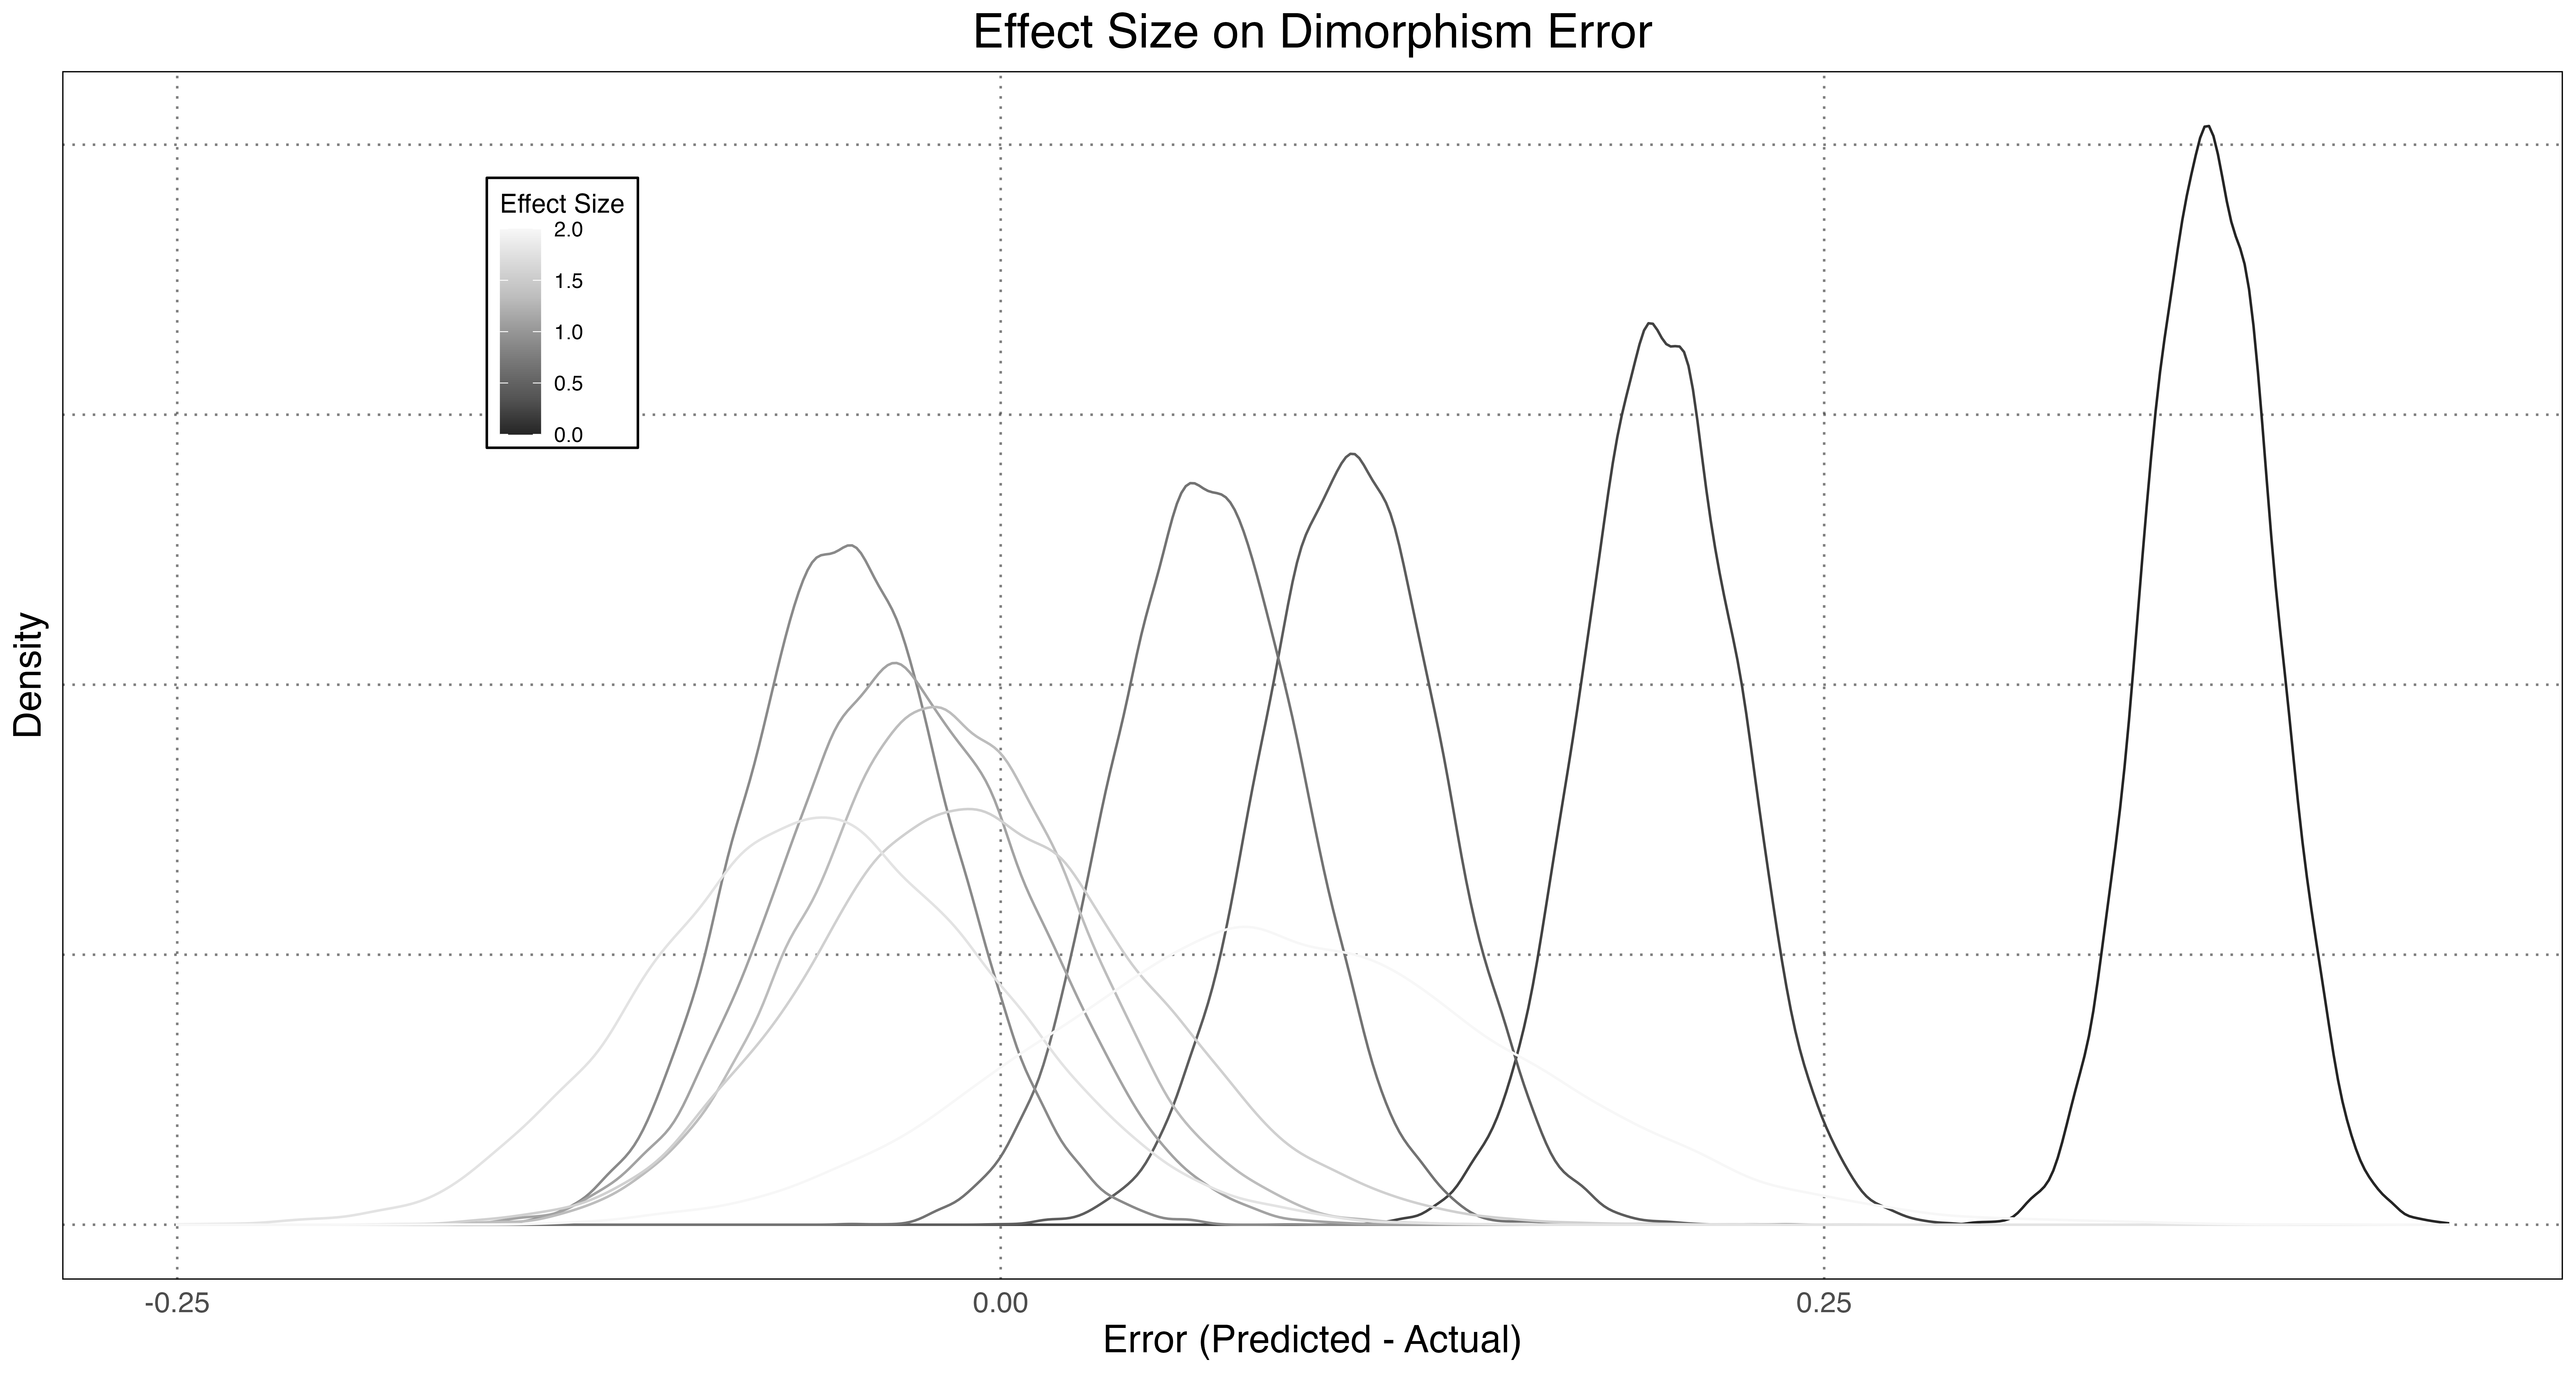
\includegraphics[width = 0.4\colwidth]{images/alligatorEffectSize-poster.png}

      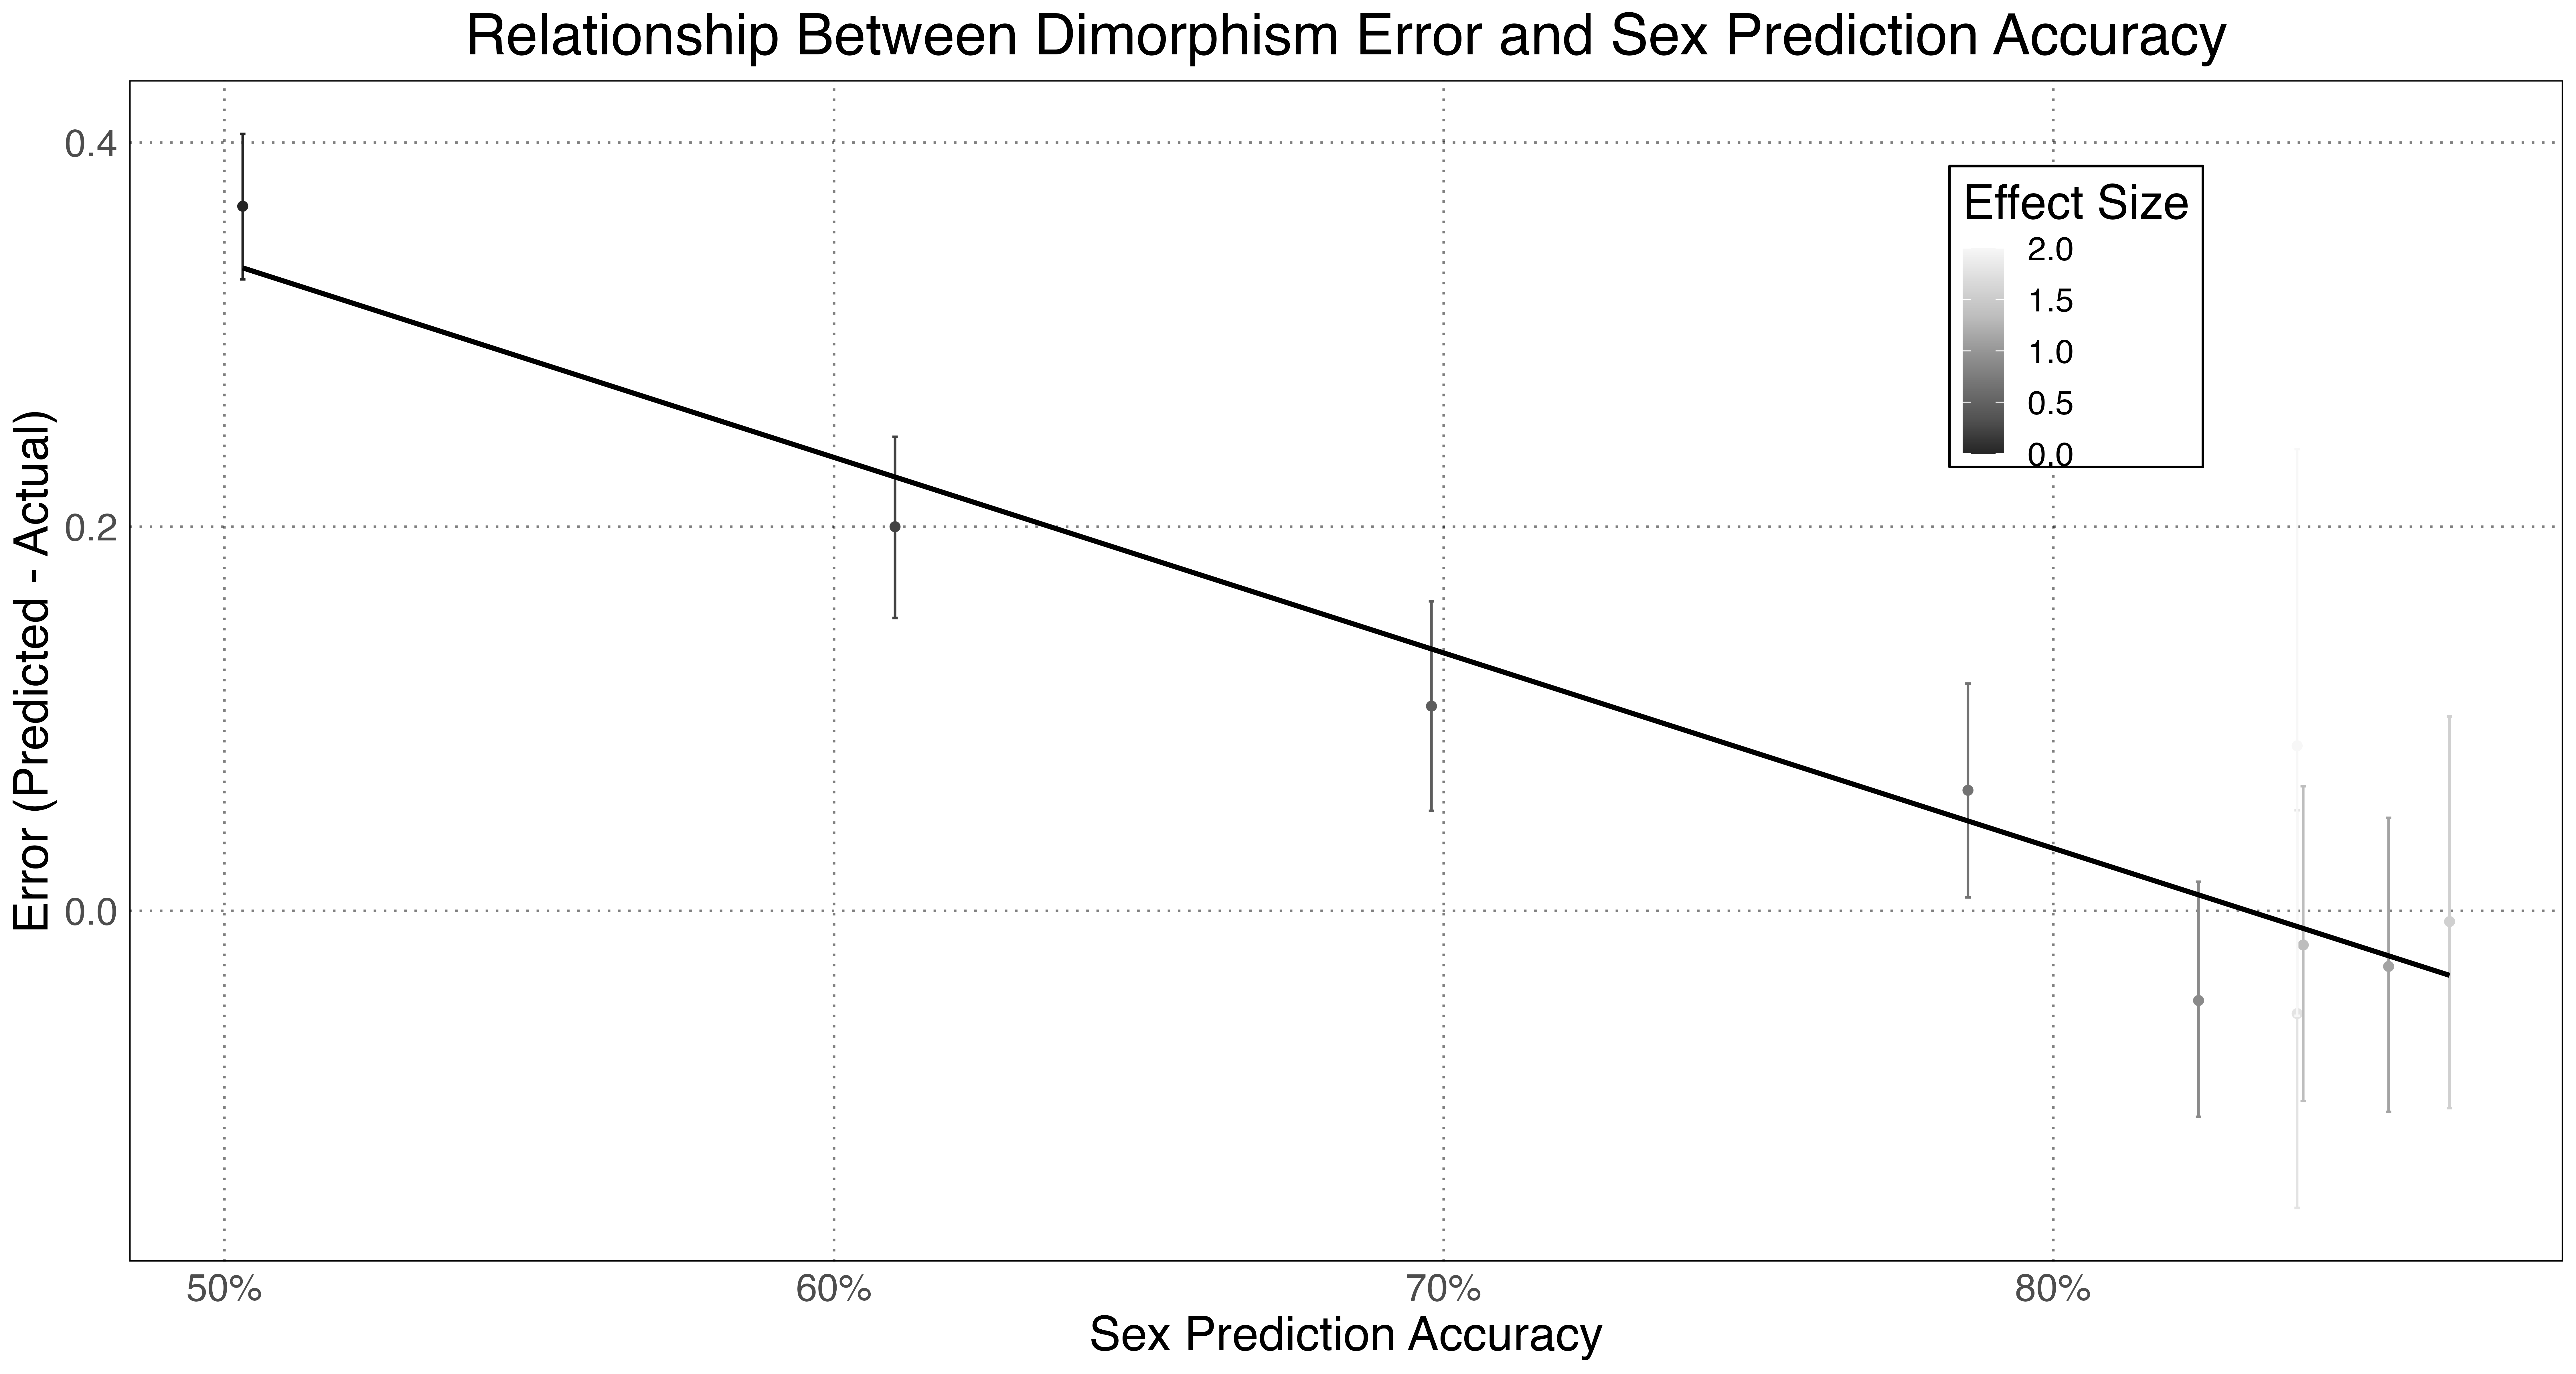
\includegraphics[width = 0.45\colwidth]{images/alligatorSexPredictionAccuracyDimorphismError-poster.png}
    \end{tikzfigure}
}

\column{0.333333333}
\block{Results}{
  \begin{itemize}
    \item \maia{}, \psit{}, and \tyran{}
    \item Logistic curve with constant standard deviation was used for all species
\[
\text{logistic}(\text{age}, L, q, k) = \frac{L}{1 + e^{q+k \ast \text{age}}}
  \]
  \end{itemize}
\begin{tikzfigure}[Posterior distribution and data]
  \centering
  \begin{minipage}[b]{0.3\colwidth}
    \centering
    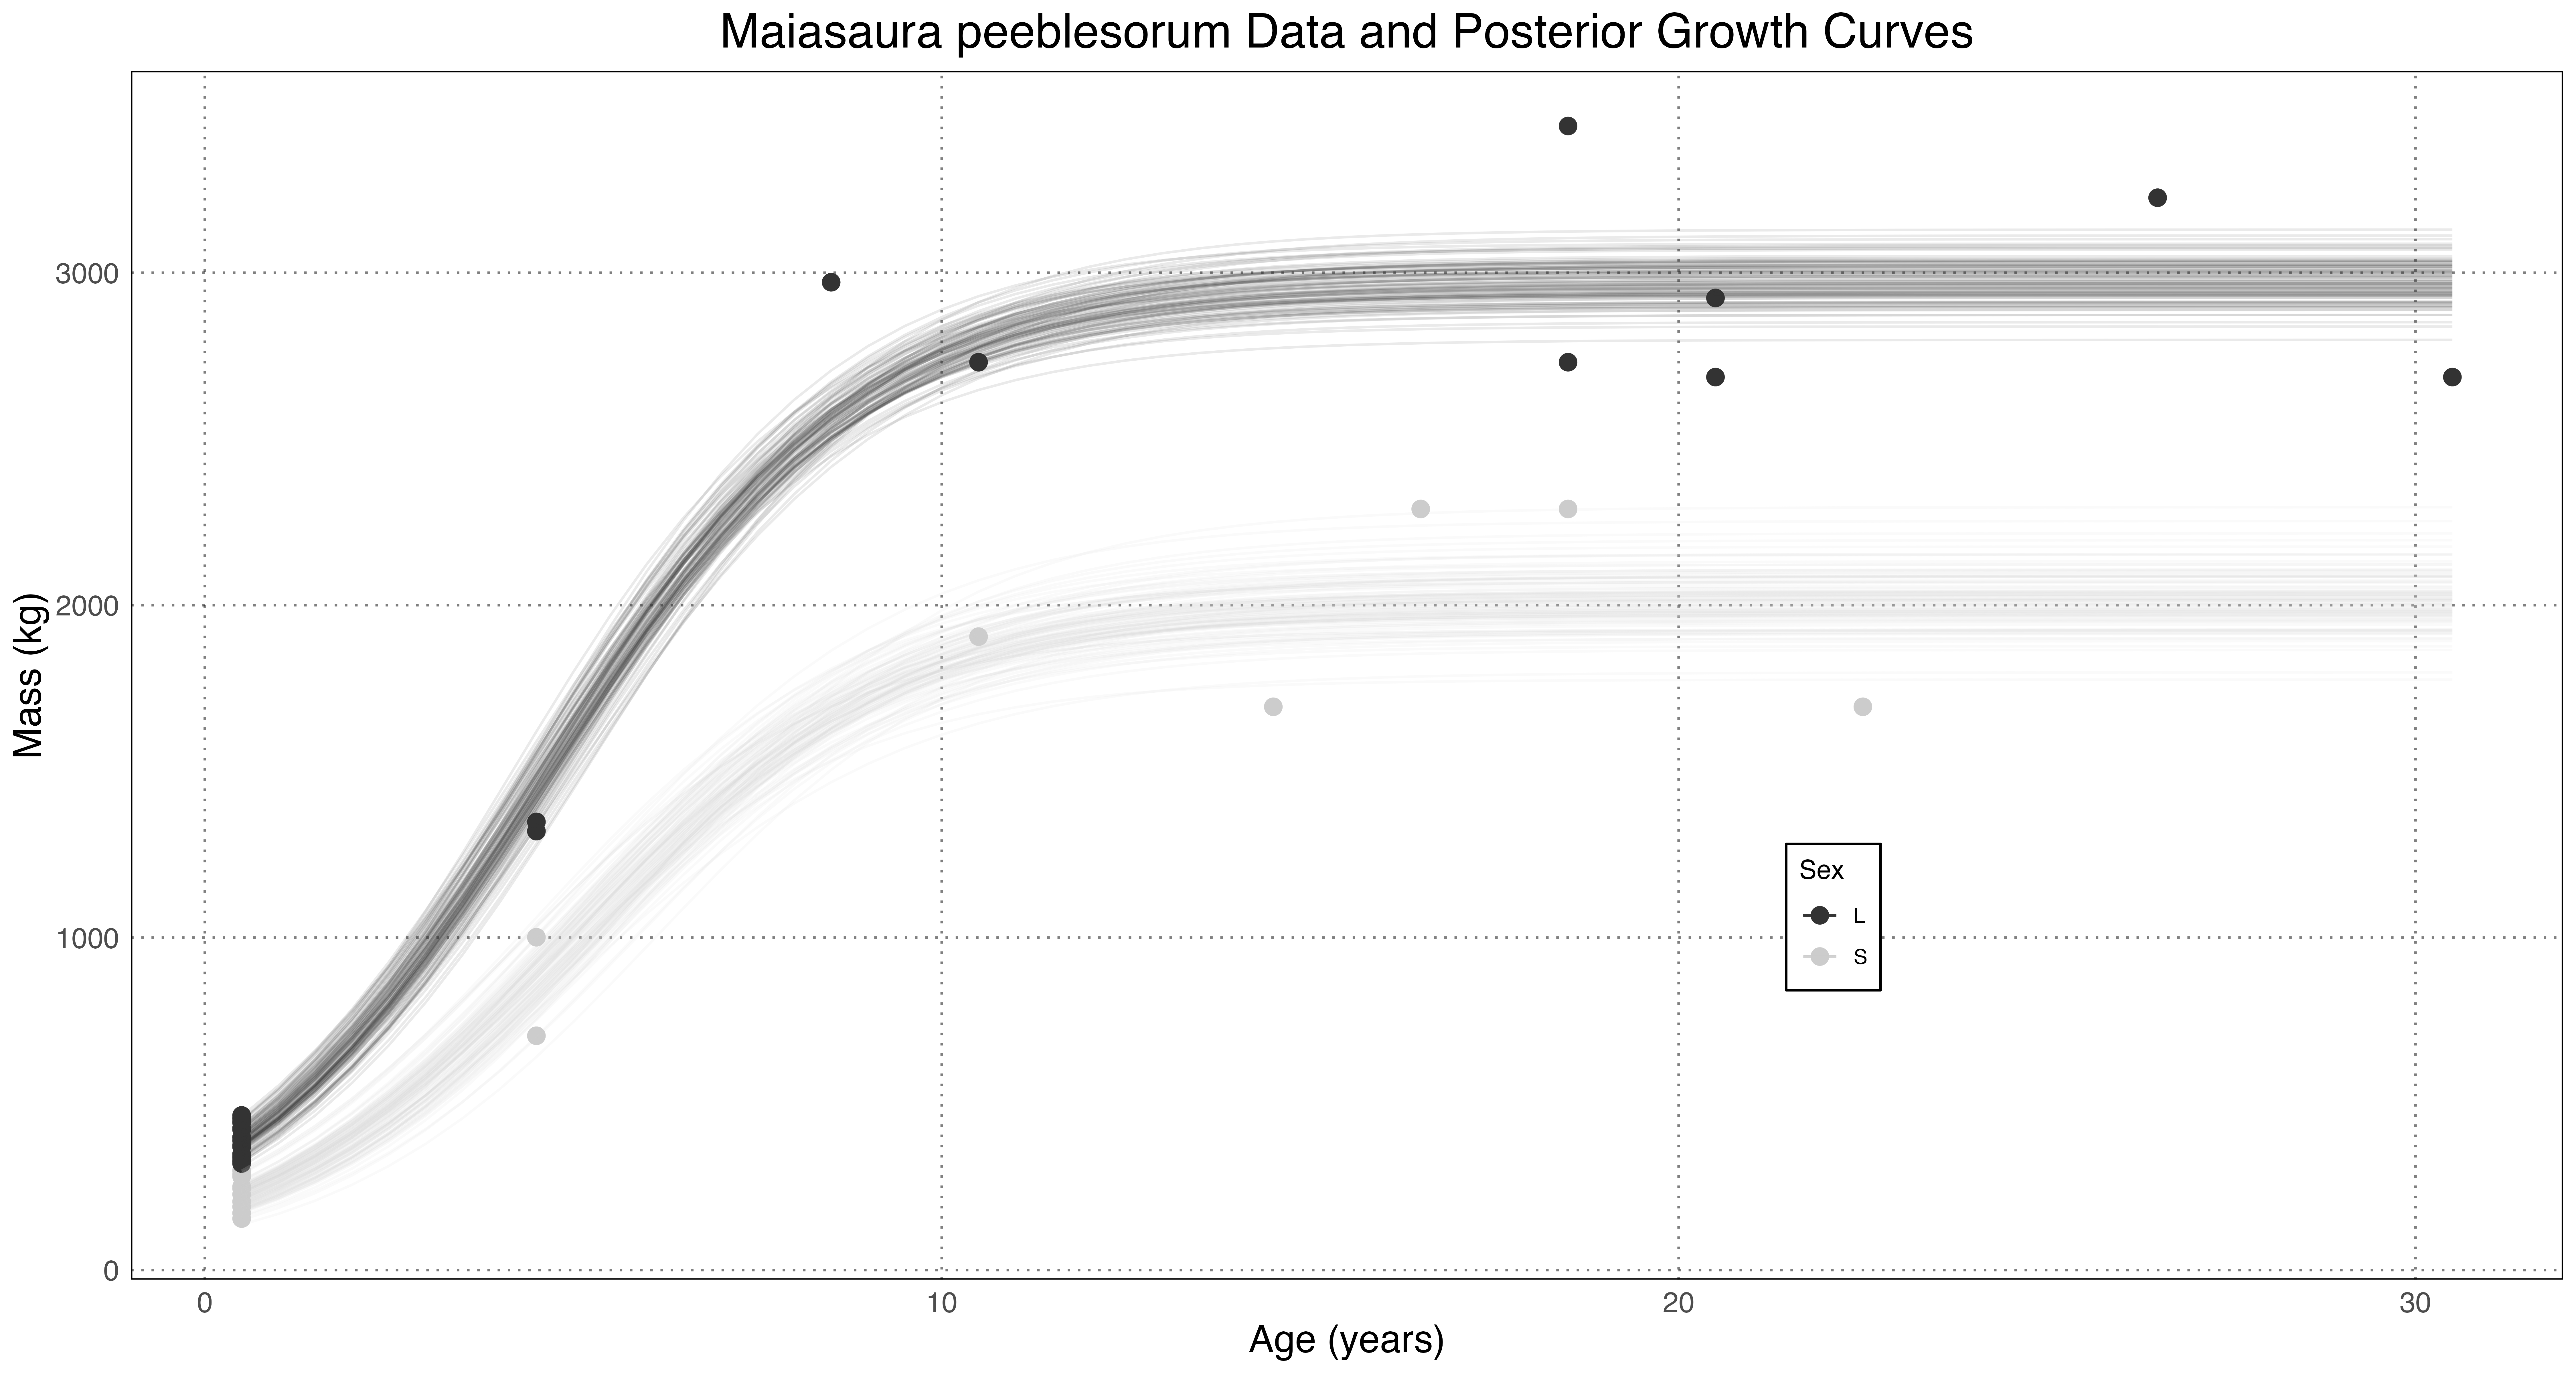
\includegraphics[width=\textwidth]{images/maiasauraPosterior-poster.png}
  \end{minipage}
  \begin{minipage}[b]{0.3\colwidth}
    \centering
    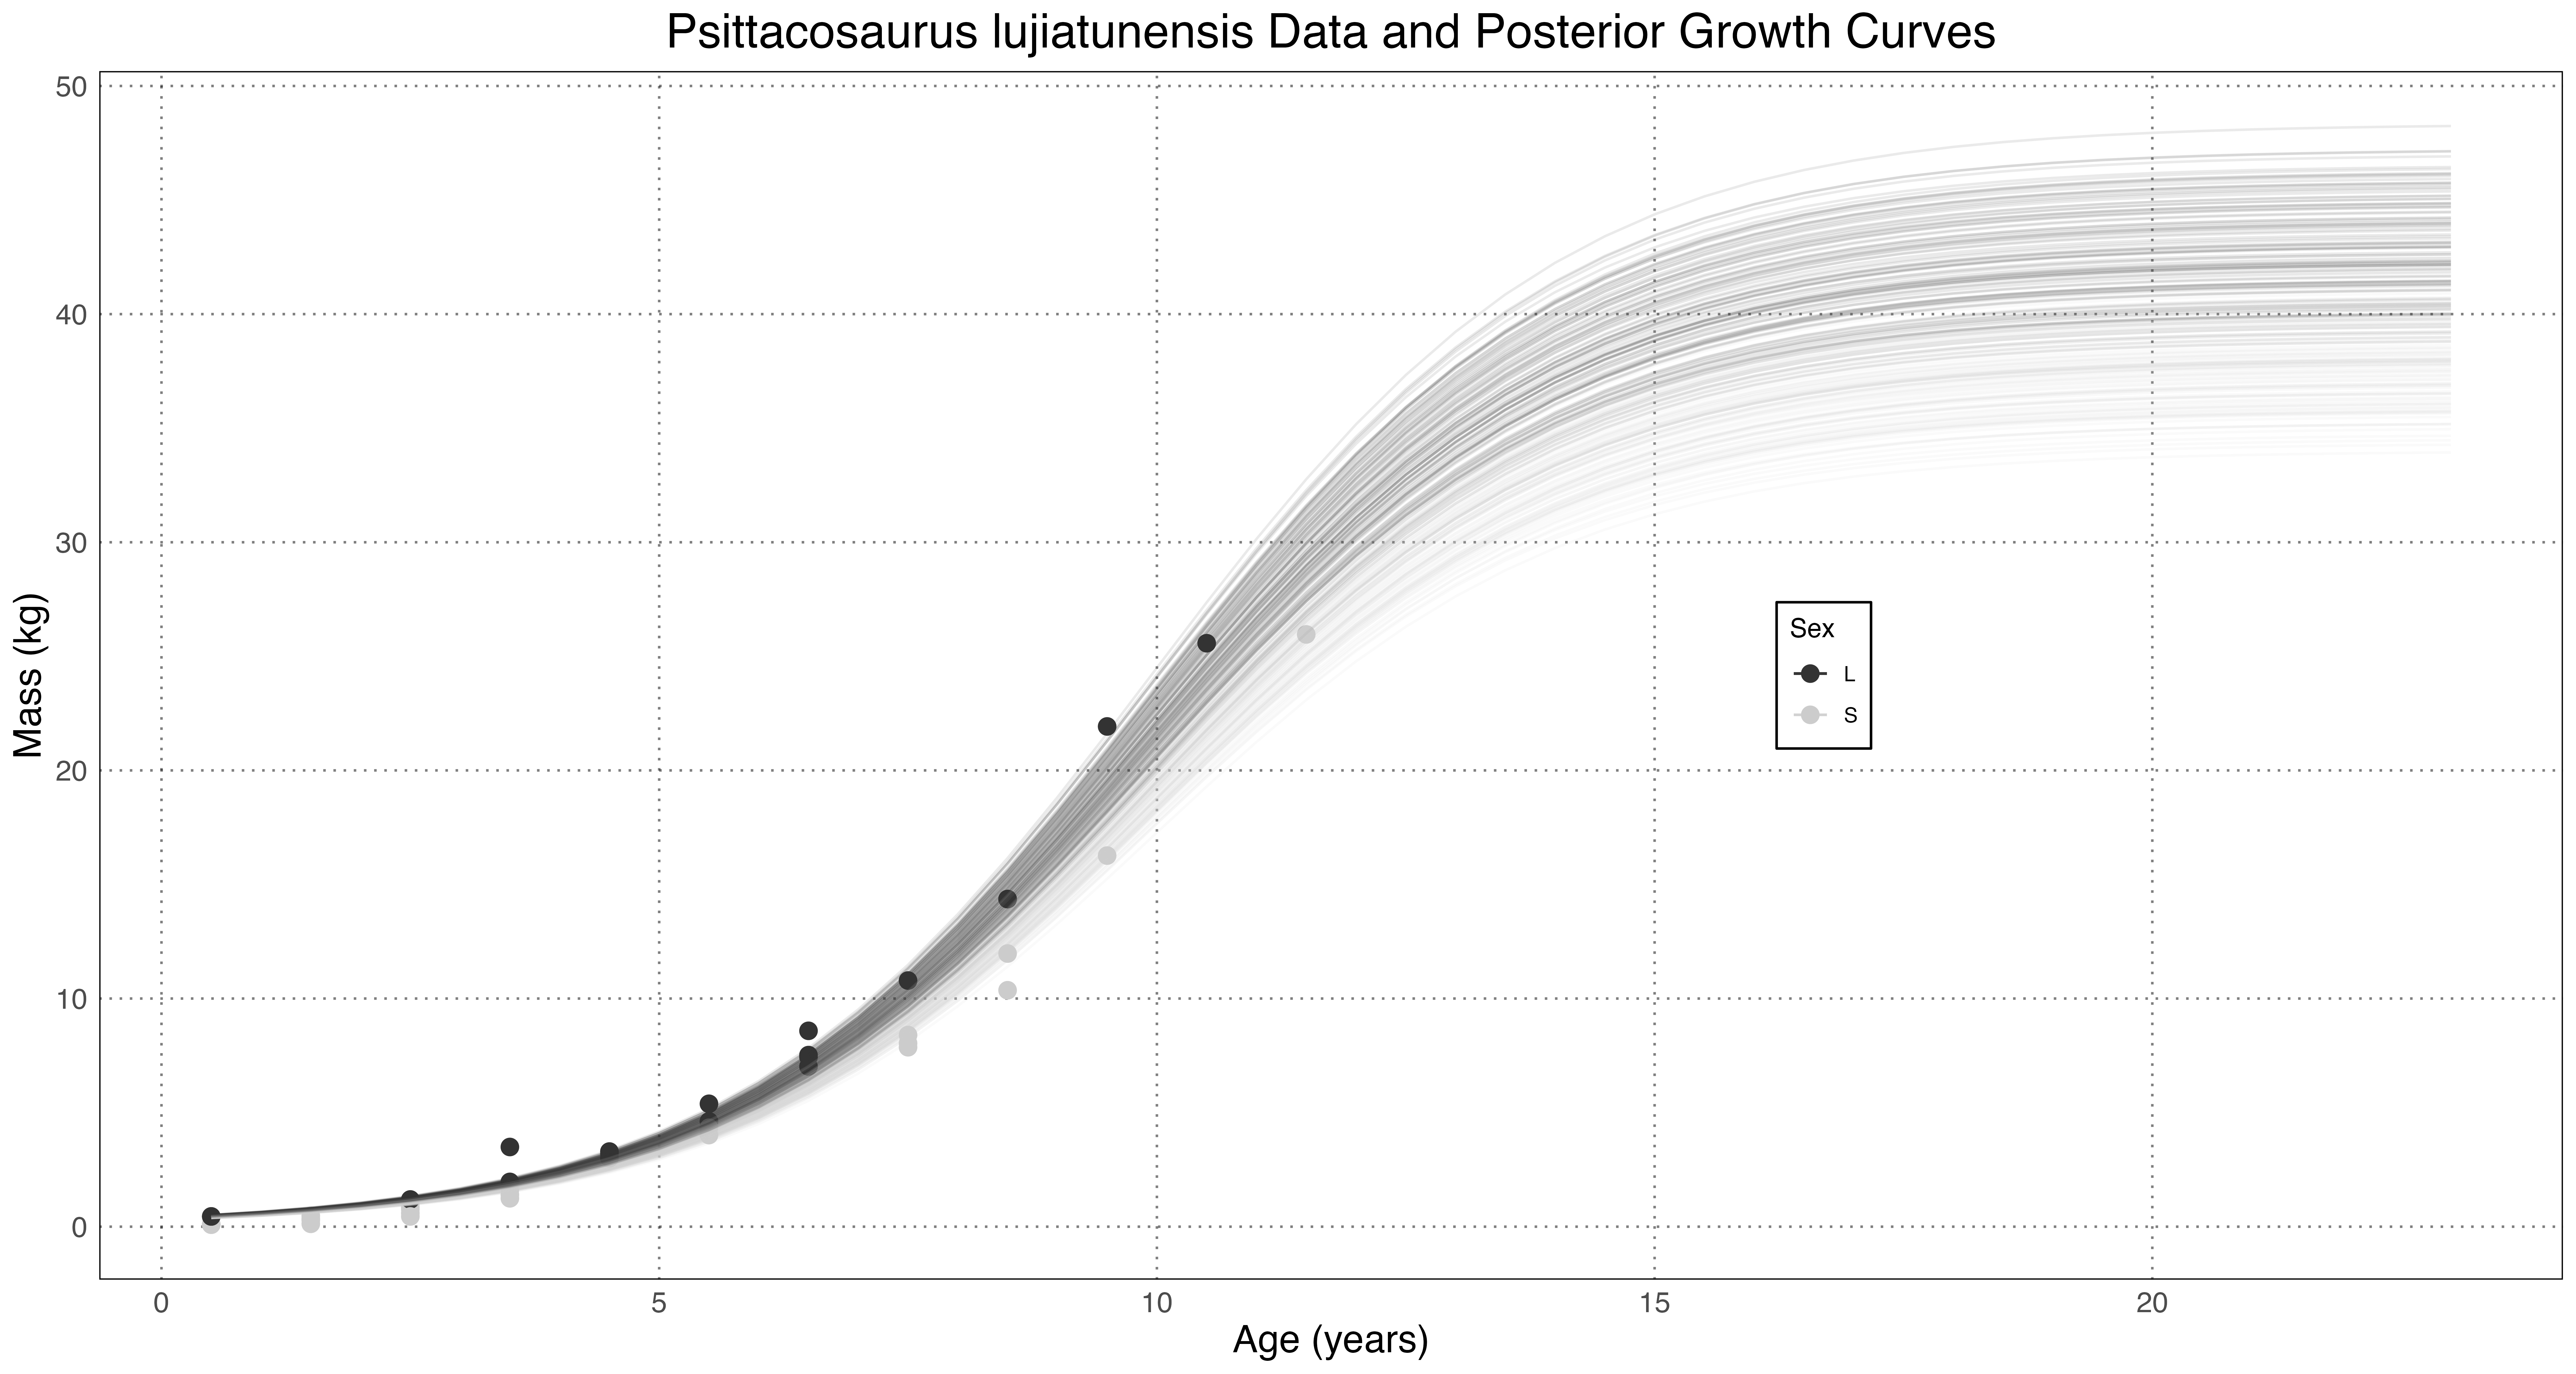
\includegraphics[width=\textwidth]{images/psittacosaurusPosterior-poster.png}
  \end{minipage}
  \begin{minipage}[b]{0.3\colwidth}
    \centering
    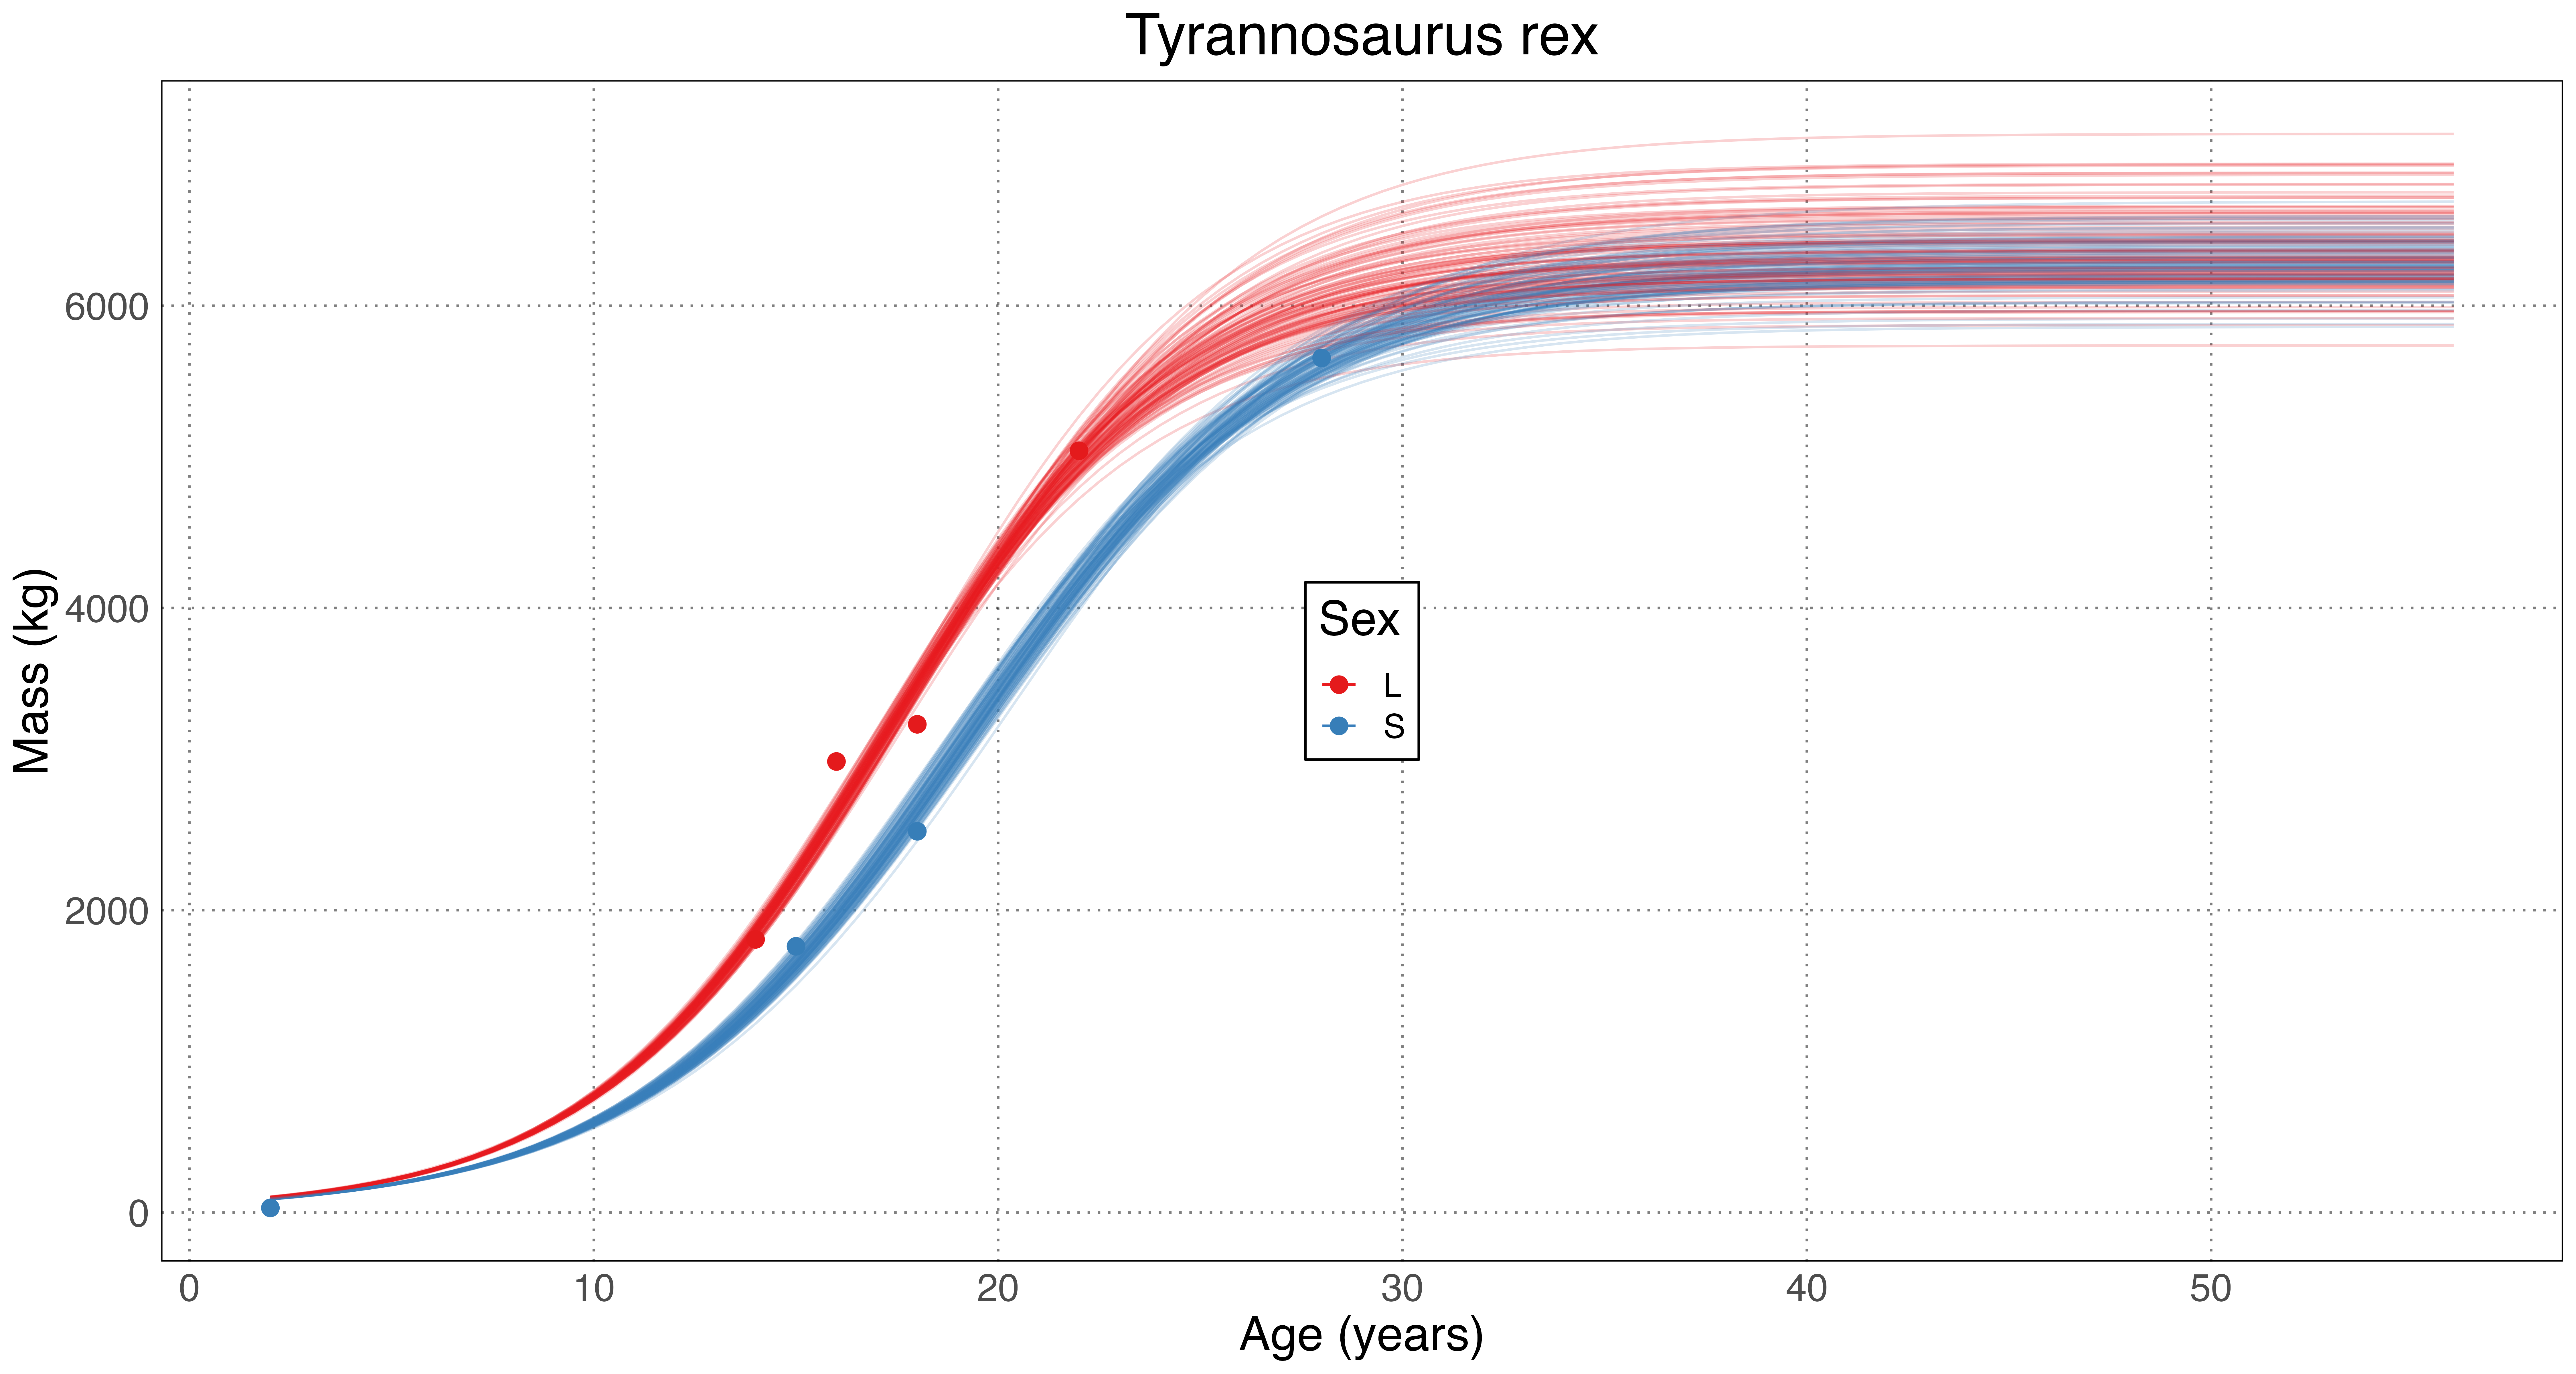
\includegraphics[width=\textwidth]{images/tyrannosaurPosterior-poster.png}
  \end{minipage}
\end{tikzfigure} 

\begin{tikzfigure}[Posterior relative dimorphism]
  \centering
  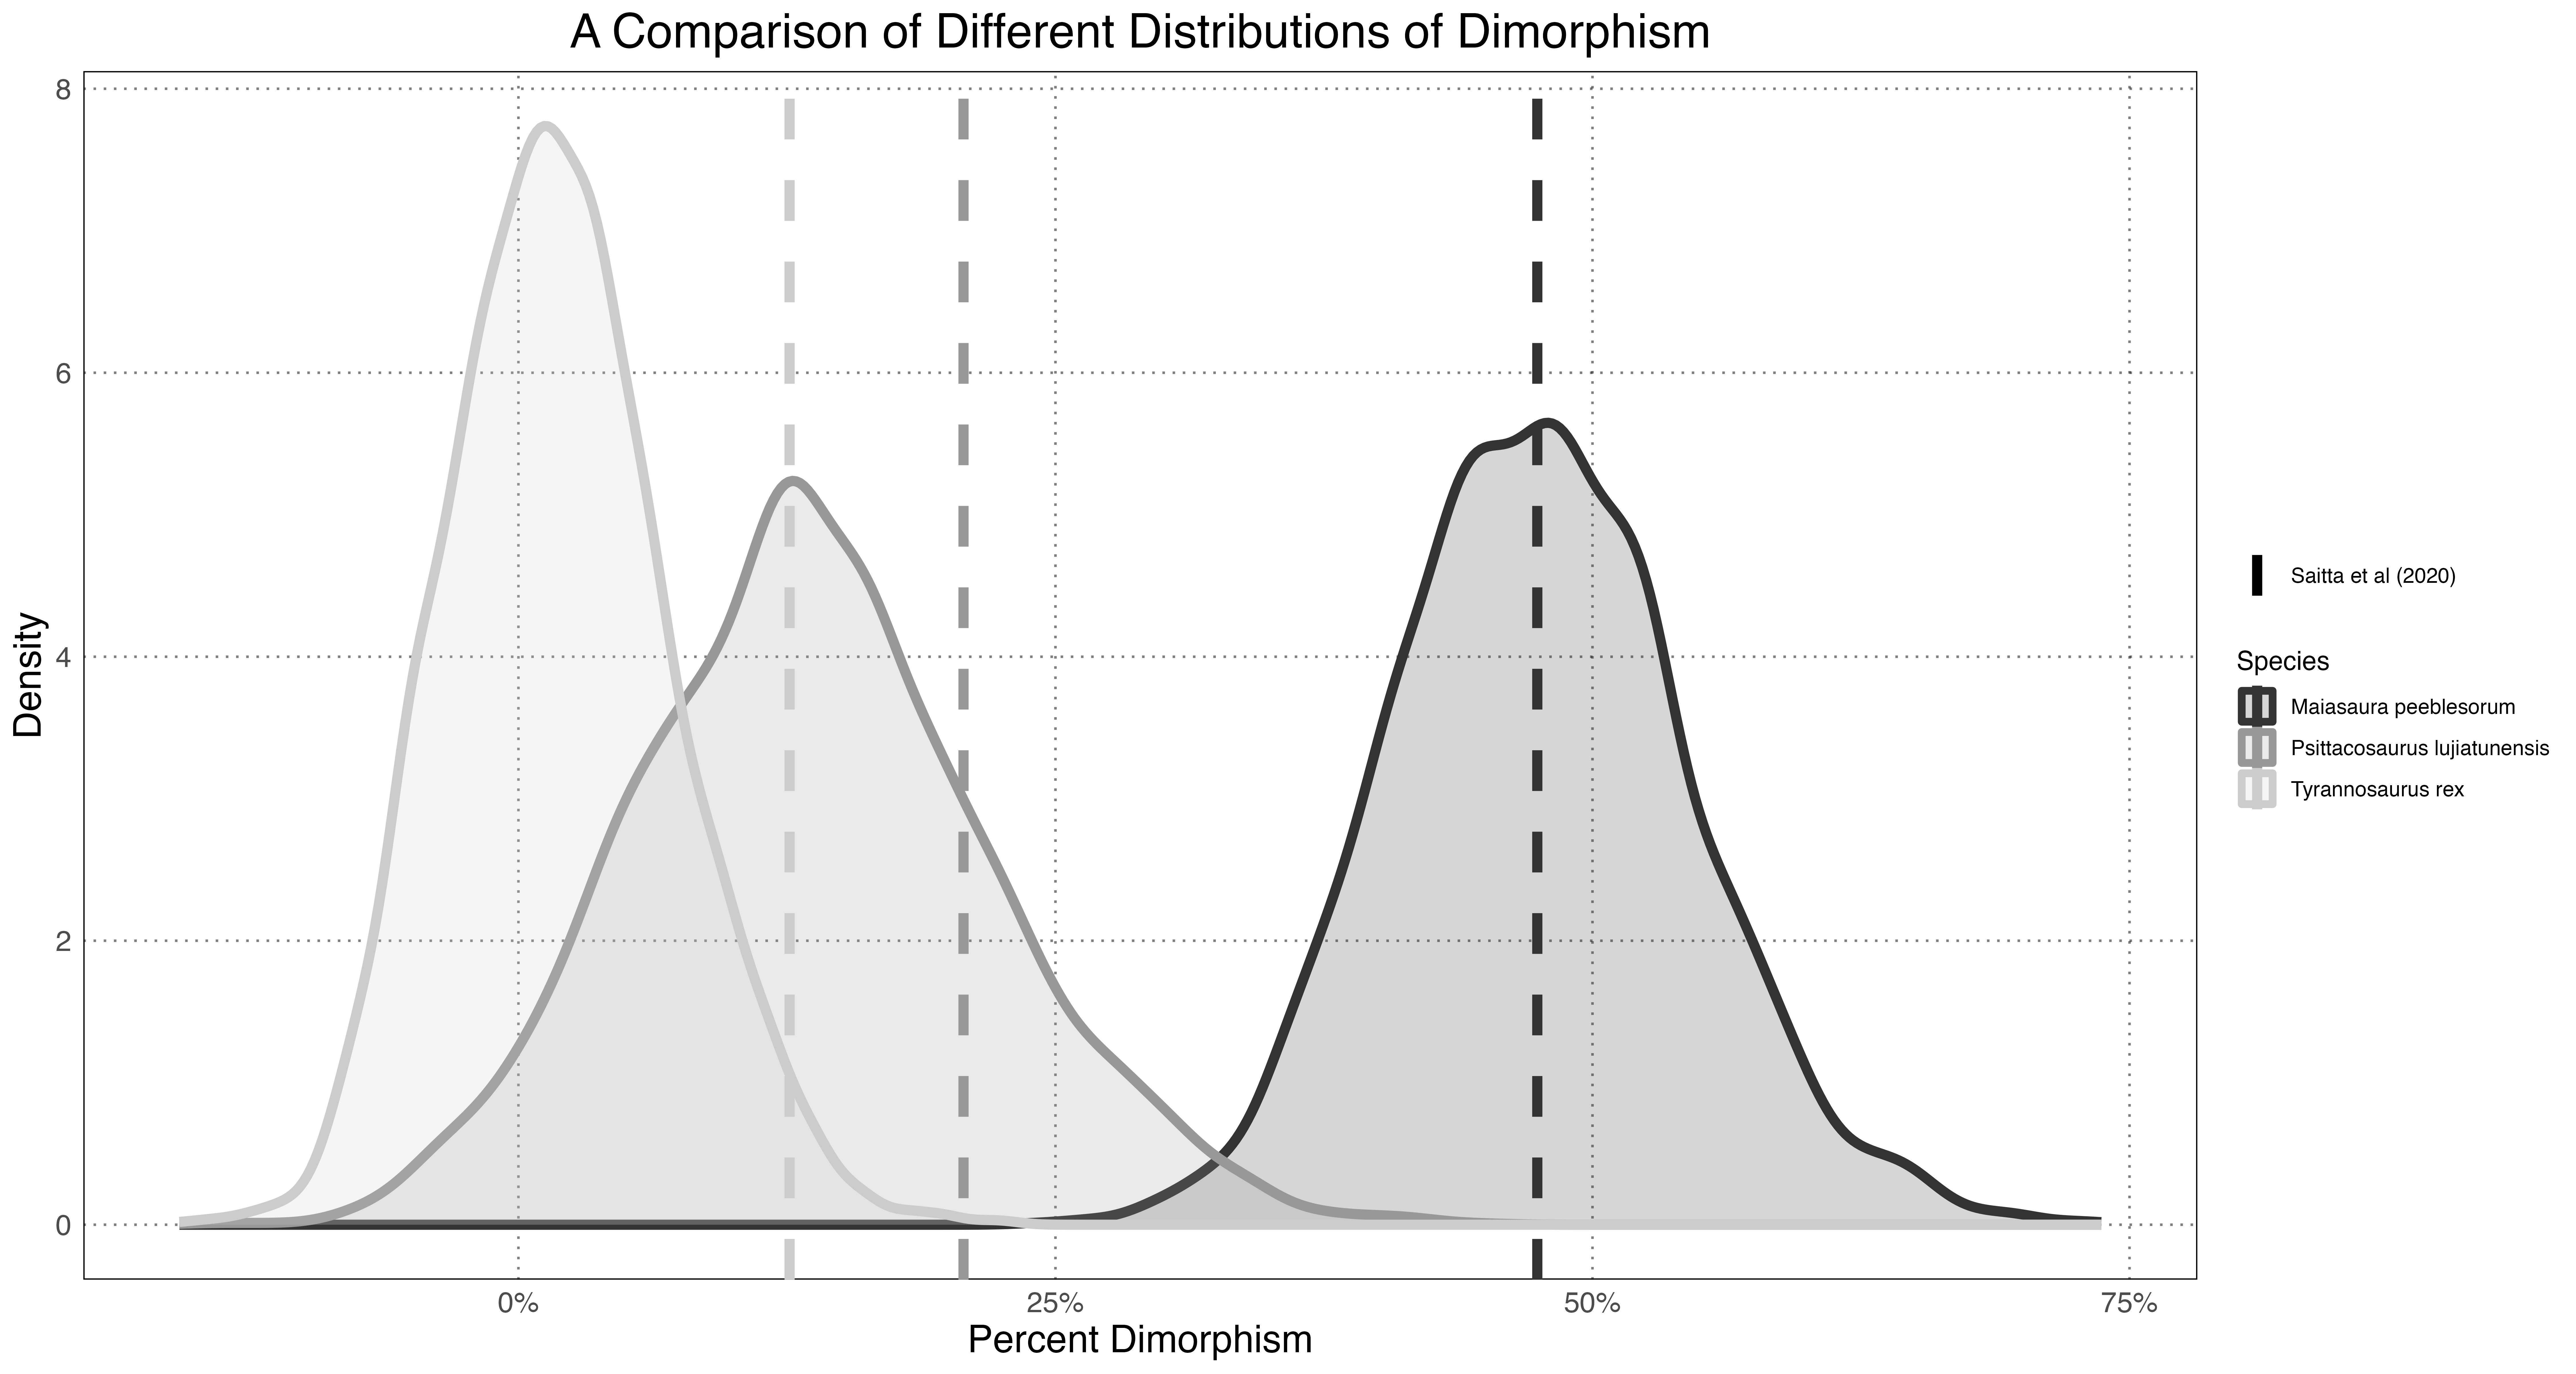
\includegraphics[width=0.9\colwidth]{images/combinedDimorphism-poster.png}
\end{tikzfigure}
  \begin{itemize}
    \item Strong evidence for \maia{} (35\% -- 62\%), weak evidence for \psit{} (-2\% -- 31\%), and moderate evidence against \tyran{} (-7\% -- 13\%) dimorphism.
    \item Benefits: incorporation of uncertainty and prior knowledge (constrain curve to be biologically feasible)
  \end{itemize}
}
\block{Next Steps}{
  \begin{itemize}
    \item Incorporate measurement uncertainty (age, size) into the model
    \item Improve sex prediction (clustering algorithms, incorporate additional features)
    \item Use of mixture models to avoid assuming dimorphism
  \end{itemize}
}
% \block{Bibliography}{
%   \nocite{saittaEffectSizeStatistical2020}
%   \nocite{brusatte2012}
%   \nocite{mallonRecognizingSexualDimorphism2017}
%   \nocite{honeProtractedGrowthImpedes2017}
%   \nocite{wilkinsonGrowthRatesAmerican1997}
%   \nocite{mcelreathStatisticalRethinkingBayesian2020}
%   \nocite{rCore, rstan}
%   % \nocite{rstan}
%   \nocite{woodwardMaiasauraModelOrganism2015}
%   \nocite{ericksonFlawedAnalysisResponse2015}
%   \nocite{ericksonGigantismComparativeLifehistory2004}
%   \nocite{hornerAgeGrowthDynamics2004}
%   \nocite{leeSexualMaturityGrowing2008}
%   \nocite{hartiganDipTestUnimodality1985}
%     \begin{minipage}{\linewidth}
%         \begin{center}\mbox{}\vspace{0pt}
%             \printbibliography[heading=none]
%         \end{center}
%         \vspace{\baselineskip}
%     \end{minipage}

%     For all data and code used here, along with additional analyses, see \url{https://github.com/EricRobertCampbell/aps-2024-poster-sexual-dimorphism}.
% }

\end{columns}
\end{document}
